% IEEE-style conference layout: 10 pt Times, two columns, US Letter.
% Main_IEEEtran.tex offers the same content with the official publisher class.
\documentclass[10pt,twocolumn,letterpaper]{article}
\usepackage[left=0.625in,right=0.625in,top=0.75in,bottom=1in,columnsep=0.25in]{geometry}
\usepackage[T1]{fontenc}
\usepackage{lmodern,times}
\renewcommand{\ttdefault}{lmtt}
\usepackage{graphicx,booktabs,array,microtype,titlesec}
\usepackage[hidelinks]{hyperref}
\graphicspath{{figures/}{../results/}}
\setlength{\parindent}{1em}\setlength{\parskip}{0pt}
\titleformat{\section}{\centering\normalsize\scshape}{\Roman{section}.}{0.5em}{}
\titleformat{\subsection}{\normalsize\itshape}{\Alph{subsection}.}{0.5em}{}
\titlespacing*{\section}{0pt}{10pt}{5pt}
\titlespacing*{\subsection}{0pt}{7pt}{3pt}
\title{\vspace{-14pt}\fontsize{23}{26}\selectfont Temporal Robustness of Graph and Tabular Models\\for Illicit Bitcoin Transaction Detection}
\author{Alex (GitHub: alexchooys)\\\small Applied Data Science, University of Florida\\\small\url{https://github.com/alexchooys}}
\date{}
\begin{document}\maketitle
\begin{abstract}
This preliminary implementation compares XGBoost, a multilayer perceptron (MLP), and GraphSAGE under four temporal adaptation policies on the original Elliptic dataset. A working Colab pipeline loads real transactions, trains the models, selects thresholds on historical validation data, and evaluates twelve model--policy combinations over fifteen later snapshots. For seed 0, recency-weighted XGBoost reaches mean post-event average precision (AP) of 0.4053, compared with 0.1983 for expanding-history retraining. Corresponding gains are smaller for the neural models. Sustained F1 recovery is not observed by the final snapshot under a predeclared support-aware rule. An interactive web prototype separates inspection of saved experiments from live inference with the frozen XGBoost checkpoint. Evidence includes executed training, a prediction-level metric audit, interface-backend tests, browser screenshots, and inference parity on 50 actual test transactions. Findings are limited to one seed and selectively labeled retrospective snapshots.
\end{abstract}
\noindent\textit{Index Terms---}anti-money laundering, GraphSAGE, distribution shift, temporal adaptation, label bias.

\section{Project Summary}
Financial-crime investigators must prioritize suspicious activity despite changing transaction patterns and limited review capacity. Graph models incorporate relationships that local-feature classifiers do not explicitly represent, but their additional complexity must be justified empirically. The original Elliptic paper already compared graph convolutional and tree models and documented deterioration around a dark-market shutdown at time step 43 \cite{weber}. Repeating that ranking or reproducing the drop alone is not the contribution of this project.

The revised question is whether graph, non-graph neural, and tree models differ in robustness and benefit differently from recent-data adaptation. Three families are crossed with frozen, expanding-history, rolling-window, and recency-weighted policies. Expanding history controls for receiving additional labels, helping separate recency effects from increasing the training set. The required MLP control helps distinguish neural modeling from explicit graph learning.

Since Deliverable 1, the real data have been loaded and validated in Colab, all three models have been trained, and all twelve seed-0 combinations have produced predictions. Implemented components include class weighting, validation-selected checkpoints and thresholds, past-only adaptive refits, timing logs, and temporal plots. The web backend exposes both saved-result inspection and frozen-tree inference. The browser interface and actual-feature inference have also been verified. Additional seeds and broader sensitivity analysis remain next steps. This is a research prototype, not a production compliance system.

\section{System Architecture and Pipeline}
\subsection{Data and Preprocessing}
The original release \cite{dataset} contains 203,769 transaction nodes, 234,355 directed payment-flow edges, and 49 snapshots. There are 4,545 illicit, 42,019 licit, and 157,205 unknown transactions. Labels associate transactions with entity categories; they do not legally establish money laundering for every transaction. Unknown targets are never recoded as licit.

Each node has 166 attributes: time step, 93 other local numerical features, and 72 supplied neighborhood aggregates. The primary predictors are the 93 local numerical values, excluding ID, time, labels, and aggregates. Neural inputs use a standard scaler fitted only to labeled training nodes from steps 1--30, held fixed afterward. Trees receive the original released values without this scaler.

The loader aligns records by transaction ID and verifies duplicates, finite values, edge endpoints, and snapshot boundaries. The observed graph has no cross-step edges. GraphSAGE retains unknown nodes as feature and edge context but excludes their targets from loss. Training and validation graphs are separately constructed. Their respective sizes are 123,287 nodes/142,784 edges and 12,978 nodes/14,059 edges; the test graph has 67,504 nodes and 77,512 edges.

\begin{table}[t]\caption{Observed known-label temporal split.}\centering\small
\begin{tabular}{lrrr}\toprule
Partition & Steps & Illicit & Licit\\\midrule
Training & 1--30 & 2,954 & 23,951\\
Validation & 31--34 & 508 & 2,481\\
Testing & 35--49 & 1,083 & 15,587\\\bottomrule
\end{tabular}\label{tab:split}\end{table}

\subsection{Artifact Flow}
Figure~\ref{fig:architecture} shows the implemented pipeline. Training writes checkpoints, validation settings, prediction CSVs, and per-step metrics. Interface callbacks read those versioned outputs; changing a filter never retrains a model. A separate route accepts new local features and evaluates the frozen XGBoost ensemble. Keeping these paths distinct prevents a saved-score lookup from being presented as live inference.

\begin{figure}[t]\centering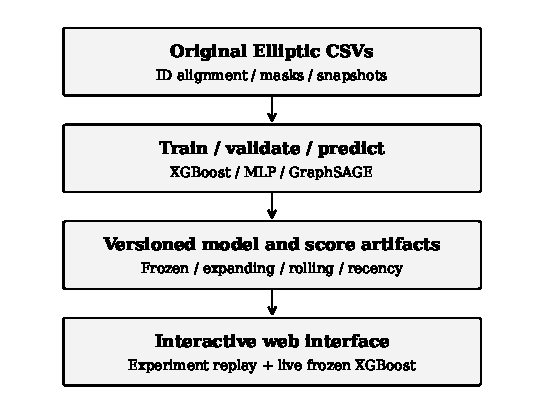
\includegraphics[width=\columnwidth]{architecture.pdf}
\caption{Implemented artifact flow. All experiments support replay; live inference currently supports frozen XGBoost.}\label{fig:architecture}\end{figure}

\section{Model Implementation Details}
\subsection{Environment and Architectures}
The executed Colab notebook records Python 3.13.16, PyTorch 2.14.1 with CUDA 13.0, PyTorch Geometric 2.8.1, and XGBoost 3.4.1. Training uses a Tesla T4 with about 14.6 GB GPU memory. These are measured environment versions, not a guarantee that identical installations are available on every system. pandas and NumPy handle data processing; scikit-learn supplies scaling and metrics.

XGBoost \cite{xgboost} uses 150 trees, depth 4, learning rate 0.05, histogram construction, and CUDA. The MLP contains two 64-unit ReLU hidden layers, dropout 0.2, and one output logit, totaling 10,241 parameters. GraphSAGE \cite{sage} uses two mean-aggregation layers, 64 hidden units, ReLU, dropout 0.2, and a linear output, totaling 20,289 parameters. Incoming directed edges are retained without automatic symmetrization. The differing parameter counts remain a limitation when attributing differences exclusively to graph structure.

Both neural models use full-batch Adam, learning rate 0.001, and weight decay $10^{-4}$. Initial training permits 200 epochs with patience 25 based on validation AP. MLP selects epoch 145 and stops at 170; GraphSAGE selects 73 and stops at 98. Binary cross-entropy uses positive-class weight 8.107989, the training negative-to-positive ratio. The same ratio defines the tree class weight and remains fixed across policies.

\begin{table}[t]\caption{Frozen validation and initial training.}\centering\small
\begin{tabular}{lrrr}\toprule
Model & Val. AP & Threshold & Seconds\\\midrule
XGBoost & .9634 & .70 & 1.51\\
MLP & .8800 & .80 & 1.67\\
GraphSAGE & .8164 & .85 & 2.11\\\bottomrule
\end{tabular}
\par\vspace{3pt}\footnotesize Neural timings include validation; tree timing measures its initial fit. These are different workloads.
\end{table}

Thresholds maximize pooled validation F1 over 0.05--0.95 in steps of 0.05, preferring the larger threshold on ties. Each model's chosen threshold is held fixed across adaptation policies. Step 32 contributes 342 of the 508 validation illicit labels, making threshold selection particularly dependent on that period. No test labels select checkpoints or thresholds.

\subsection{Adaptive Training Protocol}
When scoring step $t$, adaptive models refit from scratch on eligible known labels strictly before $t$. Predictions for $t$ are recorded before its existing known labels become eligible for $t+1$. This is a simulated one-step delay; the release does not establish real investigation turnaround. Unknown nodes never acquire invented labels.

Frozen models retain training on 1--30. Expanding uses all available historical labels, while rolling uses the previous eight snapshots. Recency uses all historical labels with weights $2^{-((t-1)-s)/4}$ for step $s$, normalized to mean one. These multiply the class-weighted loss. Adaptive neural fits use fixed 145- and 73-epoch budgets, without test-based early stopping. Graph context is confined to the permitted history; weights are checked against labeled graph-node ordering.

At $t=35$, adaptive models can use historical validation labels through 34. Frozen-to-adaptive gains therefore mix adaptation with access to additional labels. The primary recency comparison uses expanding as its control. Full-snapshot graph information is retrospective; it does not establish that every neighbor is available at transaction arrival.

\subsection{Reproducibility Checks}
The repository preserves the executed notebook and original result files. Modules cover validation, architectures, frozen-model reproduction, inference, and auditing. Recomputing AP, precision, recall, F1, and review-budget metrics from 200,040 saved prediction rows reproduces all 180 model--policy--step results. Transaction IDs and labels also match across policies. The notebook contains no saved error outputs. This is artifact verification, not an independent repeat of GPU training.

\section{Interface Prototype}
\subsection{User Interaction}
A FastAPI backend serves an HTML/JavaScript interface, providing an equivalent Python web-interface approach to Flask. The experiment explorer accepts model family, policy, time step 35--49, and a review-budget percentage. It displays AP, F1, support, budget precision/recall, a temporal chart, and a ranked transaction queue. Small illicit counts trigger a warning. The queue and metrics concern known labels; an operational precision estimate over unknown nodes is not claimed.

\begin{figure*}[t]\centering
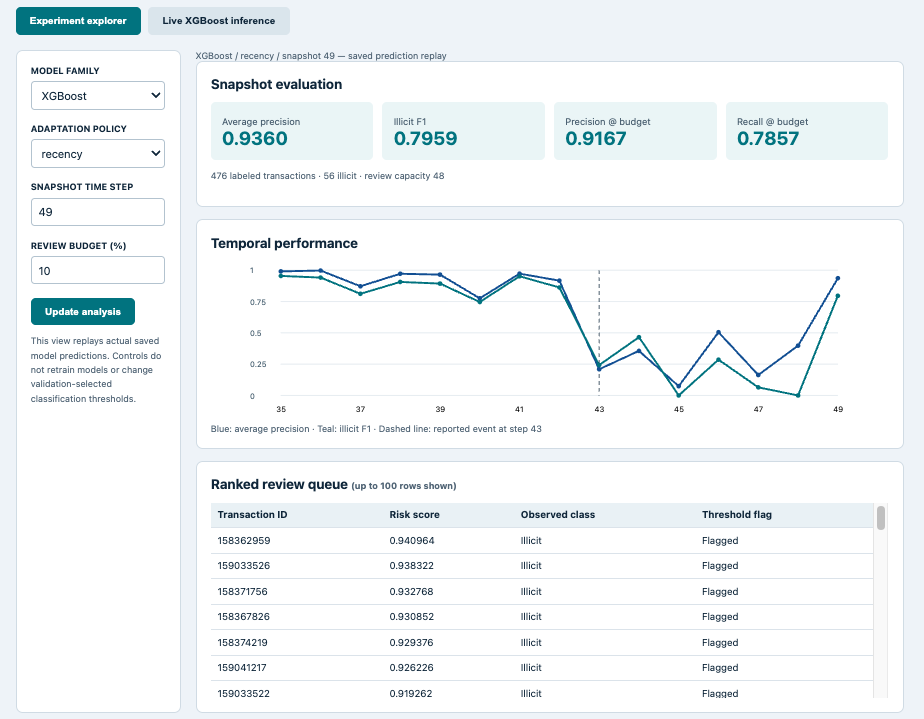
\includegraphics[width=0.49\textwidth]{interface_explorer.png}\hfill
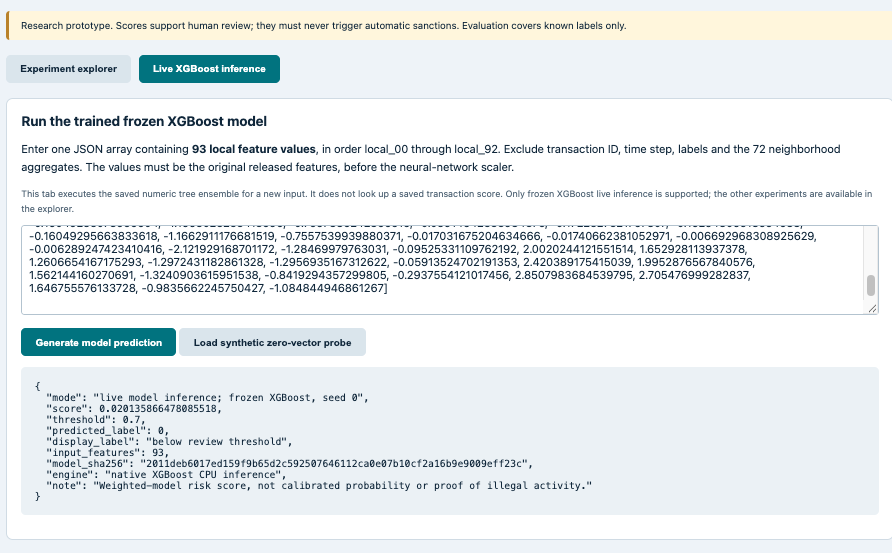
\includegraphics[width=0.49\textwidth]{interface_live_real.png}
\caption{Executed browser prototype in Colab. Left: saved XGBoost/recency results at step 49, including a temporal chart and ranked review queue. Right: live native-XGBoost inference on 93 real feature values. The explorer replays saved predictions; the live tab evaluates the frozen checkpoint.}\label{fig:ui}\end{figure*}

A separate live tab accepts exactly 93 finite feature values in local\_00--local\_92 order. Inputs exclude ID, time, target, and aggregates and must not be transformed by the neural scaler. The response reports the frozen XGBoost score, threshold 0.70, review flag, inference engine, and checkpoint hash. Native XGBoost is used when installed. A restricted numerical-tree evaluator supports lightweight use and rejects categorical or unsupported models. A Colab verification cell compares the engines on actual feature rows and saved scores.

\subsection{Executed Outputs and Limits}
The explorer selection XGBoost/recency/49 reproduces AP 0.9360 and F1 0.7959 across 476 known-label transactions, including 56 illicit. At a 10\% review budget, 48 transactions are selected: precision is 0.9167 and recall is 0.7857. These budget metrics differ from the validation-threshold precision and recall. Figure~\ref{fig:ui} shows the rendered explorer and live tab.

The executed Colab demo checks the first 50 saved test transactions after aligning their original feature rows by transaction ID. Maximum absolute differences are $2.935\times10^{-8}$ between native XGBoost and stored scores and $5.974\times10^{-8}$ between the portable evaluator and native XGBoost. Both pass the prewritten absolute/relative tolerance of $10^{-5}$. This verifies inference consistency on those rows, not retraining reproducibility or population-wide equivalence.

A real 93-feature input produces score 0.02013587 with native XGBoost CPU inference. With threshold 0.70 the output is below review threshold, flag 0. The checkpoint SHA-256 matches the saved training artifact. This demonstrates new model evaluation rather than a stored-score lookup; the low score is not proof of legitimate activity.

HTTP tests cover the page, valid replay, invalid policy, low support, malformed live inputs, and a successful prediction. All 180 explorer selections pass. The executed UI notebook contains no saved errors, and the browser screenshots document rendering and outputs. Live neural inference, adaptive checkpoint serving, and unknown-node review are not yet integrated.

\section{Early Evaluation and Results}
\subsection{Metrics and Frozen Performance}
AP denotes average precision, not trapezoidal PR-AUC. Additional metrics include per-step illicit precision, recall, F1, support, and precision/recall among the highest-scoring 10\% of known-label transactions. Phase results equally average per-step metrics over 35--42 and 44--49, with 43 reported separately. They are not pooled-transaction estimates.

Frozen XGBoost AP decreases from 0.9040 before the event to 0.0789 afterward. Corresponding MLP values are 0.7452 and 0.0938; GraphSAGE values are 0.6947 and 0.0716. Thus deterioration is visible in the real implementation. A drop does not identify its sole cause, and AP changes with prevalence and ranking difficulty. Steps 45 and 46 contain only five and two illicit nodes; isolated spikes there are especially unstable.

\begin{figure*}[t]\centering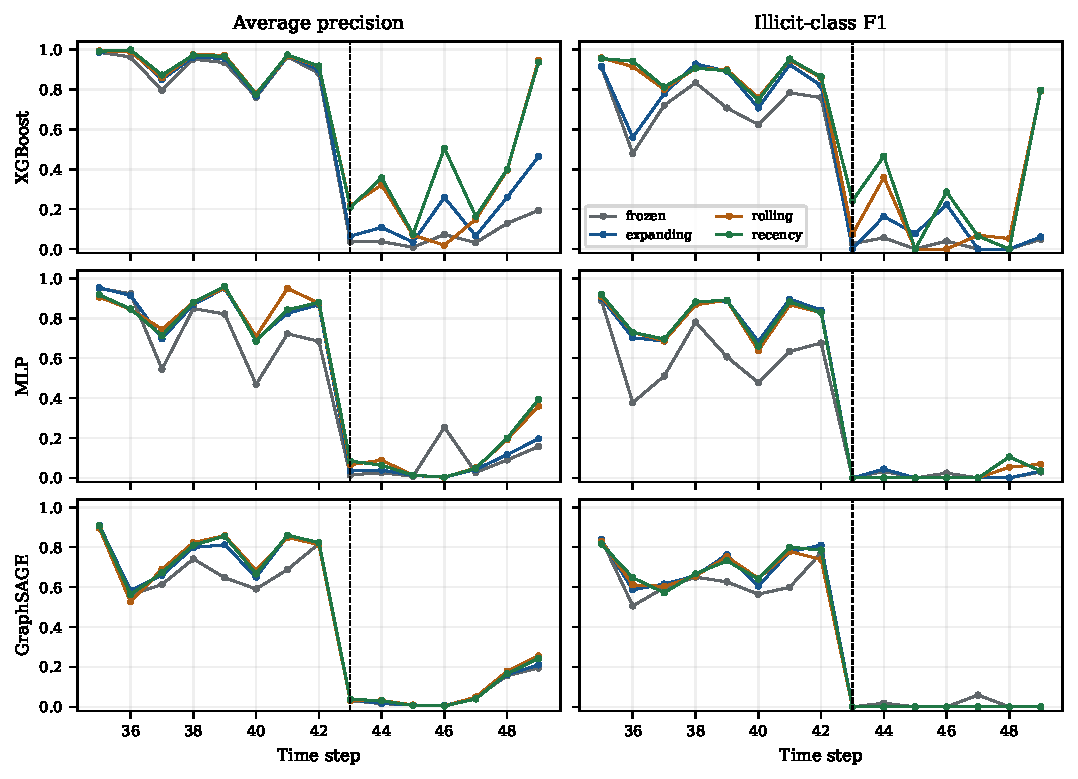
\includegraphics[width=0.96\textwidth]{adaptation.pdf}
\caption{Measured seed-0 trajectories for all twelve combinations. The dashed line marks step 43. A late one-step rebound does not establish sustained recovery.}\label{fig:results}\end{figure*}

\begin{table}[t]\caption{Mean post-event AP, steps 44--49, seed 0.}\centering\small
\begin{tabular}{lrrrr}\toprule
Model & Frozen & Expand & Rolling & Recency\\\midrule
XGBoost & .0789 & .1983 & .3164 & \textbf{.4053}\\
MLP & .0938 & .0684 & .1179 & .1203\\
GraphSAGE & .0716 & .0755 & .0881 & .0817\\\bottomrule
\end{tabular}\label{tab:results}\end{table}

\subsection{Model-by-Policy Differences}
Recency-weighted XGBoost improves post-event AP over expanding by 0.2070. Corresponding gains are 0.0519 for MLP and 0.0062 for GraphSAGE. Rolling gains are 0.1182, 0.0495, and 0.0126. Recent history therefore benefits the tree model more in this configuration. Expanding-history MLP is worse than its frozen reference, showing that additional labels alone need not improve a model.

The XGBoost-minus-GraphSAGE difference in recency gains is about 0.2008 AP. This is a descriptive model-by-policy contrast, not a statistical significance result. Model capacity, optimization and selected epoch budgets differ. More seeds and diagnostic analysis are necessary before claiming a general architecture advantage. The observed result nevertheless answers the revised question even though the graph model does not win.

Adaptive GraphSAGE has zero post-event F1 for all policies at threshold 0.85. Expanding, rolling and recency issue 41, two and three alerts, respectively; all are false positives and all 145 known illicit nodes are missed. Nonzero AP reflects score ordering even when the operating threshold misses positives. This motivates distinguishing ranking from threshold behavior, without retuning on holdout outcomes.

\subsection{Recovery and Compute}
Recovery requires two consecutive post-event steps reaching at least 90\% of that combination's mean pre-event F1, with at least ten illicit and ten licit labels in each step. Only two consecutive pairs satisfy the support requirement. Recovery is not observed by 49 for any combination. XGBoost's final-step rebound cannot qualify without a second supported step. This is limited follow-up rather than evidence of permanent failure.

For 45 adaptive refits per family, summed fit durations are 36.67 s for XGBoost, 23.42 s for MLP and 52.13 s for GraphSAGE. The notebook's full adaptation durations are 47.75, 39.81 and 81.14 s, including preprocessing, inference, metrics and repeated writes. The experiment is practical on the measured T4, although costs can change with hardware, implementation and history size. No energy or carbon estimate is inferred from these times.

\section{Challenges and Next Steps}
\subsection{Selective Labels and Short Follow-Up}
Validation labels are concentrated in one snapshot and post-event illicit support is sparse. Counts accompany metrics, and recovery explicitly permits a not-observed outcome. Initialization seeds will assess one source of variability, but cannot replace new time periods or resolve selective labeling. A temporal split evaluates transfer to later snapshots without claiming that all real deployment conditions are represented.

\subsection{Protocol and Implementation Boundaries}
Training-history masks must exclude current and future labels. Unknown targets remain masked, and graph-node ordering checks prevent incorrect recency-weight assignment. Settings are retained after viewing test results; window length, half-life and thresholds will not be selected for favorable holdout outcomes. Additional diagnostic views will be clearly separated from predictors, especially any analysis that uses observed neighbor labels.

Browser screenshots and actual-feature native-parity evidence are retained with the executed demo notebook. The updated project must be committed to GitHub, with the actual repository URL submitted alongside this report. Raw data and authentication files do not belong in that commit.

\subsection{Refinement Before Deliverable 3}
Seeds 1 and 2 will repeat initial validation selection independently and freeze each seed's choices across policies. Further work includes label-delay sensitivity, degree/isolation error analysis, and UI polish. Training-only graph embeddings for XGBoost remain optional. The next priority is assessing result stability while maintaining the implemented interface. No additional tuning will consume the current post-event results as a development set.

\section{Responsible AI Reflection}
Known illicit labels reflect activity investigators detected and attributed. They may encode investigative priorities and blind spots; unknown records may include undetected illicit behavior. Performance on observed labels therefore does not establish comprehensive laundering detection. Anonymized features prevent credible demographic fairness claims, and a favorable benchmark score cannot guarantee equitable operational treatment.

False positives can harm legitimate users. Outputs must support human review and never trigger automatic sanctions, account closure, or legal accusations. The interface separates observed classes from predictions and states that weighted-model scores are not calibrated probabilities. Re-identification is not attempted; credentials and raw input files are excluded from the repository distribution.

Transparency includes retaining unfavorable findings, including graph-model failures and absent sustained recovery. Simulated label availability and retrospective snapshot access are disclosed. Shallow networks, bounded searches and measured runtimes limit computational waste. AI assistance supported design, code generation, writing, and formatting; executed real-data outputs, artifact checks, and retained interface evidence support the reported measurements.

\begin{thebibliography}{9}
\bibitem{weber} M. Weber et al., ``Anti-Money Laundering in Bitcoin: Experimenting with Graph Convolutional Networks for Financial Forensics,'' KDD Workshop on Anomaly Detection in Finance, 2019, arXiv:1908.02591.
\bibitem{dataset} Elliptic, ``Elliptic Data Set,'' Kaggle. [Online]. Available: \url{https://www.kaggle.com/datasets/ellipticco/elliptic-data-set}.
\bibitem{xgboost} T. Chen and C. Guestrin, ``XGBoost: A Scalable Tree Boosting System,'' Proc. ACM SIGKDD, 2016, pp. 785--794.
\bibitem{sage} W. L. Hamilton, R. Ying, and J. Leskovec, ``Inductive Representation Learning on Large Graphs,'' Advances in Neural Information Processing Systems, 2017, arXiv:1706.02216.
\end{thebibliography}
\end{document}
